\chapter[Zielspezifikation und Darlegung des Forschungsdesigns]{Zielspezifikation und Darlegung des Forschungsdesigns\footnote{Sprachlich geglättet durch ChatGPT-5}}
\label{chapter:Ziel_und_Forschungsdesign}

\section{Zielsetzung}\label{sec:zielsetzung}
Ziel dieser Arbeit ist die prototypische Entwicklung und Evaluation eines IT-Artefakts in Form einer Datenpipeline zur Generierung synthetischer Bilddaten aus einem digitalen Modell einer Laserschneidmaschine in einer Simulationsumgebung. Die Pipeline soll automatisiert umfangreiche und qualitativ hochwertige Bilddatensätze erzeugen, die spezifische Fehlerzustände der Maschine abbilden. Dabei stehen die Reproduzierbarkeit des Prozesses, die Flexibilität durch Parametrisierung sowie die einfache Erweiterbarkeit um zusätzliche Fehlerzustände im Vordergrund.

Zur Validierung der Pipeline werden die erzeugten Daten exemplarisch für das Training und die Evaluation von \ac{KI}-Modellen eingesetzt. Diese Modelle bilden nicht den Hauptfokus der Arbeit, sondern dienen als Mittel, um die Eignung und Konsistenz der generierten synthetischen Daten nachzuweisen. Die Evaluation der Modelle erfolgt dabei sowohl auf synthetischen als auch realen Bilddaten. Die Arbeit versteht sich somit als \textit{Proof-of-Concept}, der die Machbarkeit und das Potenzial pipelinebasierter Datengenerierung für die \ac{KI}-gestützte Fehlererkennung in der Fertigungsindustrie aufzeigt. Erzielte Ergebnisse sollen dabei auch auf andere Domänen übertragbar sein, da der Mangel an ausreichenden und umfassenden Bilddaten für solche Anwendungen nicht ausschließlich in der Fertigungsindustrie eine Problematik darstellt.\footnote{Vgl. \cite[2]{bai_bridging_2023}}

Exemplarisch wird die Pipeline in einem konkreten Anwendungsfall eingesetzt, bei welchem erkannt werden soll, ob ein ausgeschnittenes Teil während des Betriebs einer Laserschneidmaschine noch im Blech vorhanden ist. Mit einer solchen Information kann nachgelagerten Prozessen der konkrete Fehlerfall klassifiziert und im Idealfall autonom behoben werden. Dieser Anwendungsfall dient als Demonstrator, um die Funktionsfähigkeit und den praktischen Nutzen der Pipeline im Rahmen eines \textit{Proof-of-Concepts} zu veranschaulichen.


\section{Forschungsmethodik}\label{sec:forschungsmethodik}
Zur Erreichung der in Abschnitt \ref{sec:zielsetzung} beschriebenen Zielsetzung wird das \ac{DSR}-Paradigma angewendet. Bei \ac{DSR} handelt es sich um einen anerkannten Forschungsansatz in Informationssystemen, der darauf abzielt, durch die Entwicklung und Evaluation innovativer Artefakte, Probleme in der Praxis zu lösen und gleichzeitig einen Beitrag zur wissenschaftlichen Wissensbasis zu leisten.\footnote{Vgl. \cite[S.337]{the_australian_national_university_positioning_2013}}
Im Rahmen von \ac{DSR} werden Artefakte, wie z.B. Systeme, Methoden oder Modelle entworfen und iterativ in einem \textit{Build-and-Evaluate}-Zyklus weiterentwickelt, um ihre Eignung zur Problemlösung zu überprüfen und zu verbessern.\footnote{Vgl. \cite[78]{hevner_design_2004}} Dieser Prozess umfasst die Identifikation des Problems, die Definition von Anforderungen, die Entwicklung eines Artefakts sowie dessen Demonstration, Evaluation und Kommunikation. \footnote{Vgl. \cite{peffers_design_2007}}

Das in dieser Arbeit entwickelte Artefakt besteht aus einer Pipeline zur Generierung synthetischer Bilddaten, die auf einem digitalen Modell in einer Simulationsumgebung basiert. Das Ziel ist es, die Datengrundlage für \ac{KI}-Modelle zur Fehlererkennung im Fertigungsbereich zu verbessern, insbesondere in Hinblick auf Fortschritte im Bereich des Remote Monitoring. Bereits in Abschnitt \ref{sec:synthetische_daten_section} genannte Probleme, wie Kosten- und Zeitaufwand sowie der \textit{Domain Gap} sollen durch dieses Artefakt konzeptionell adressiert werden. 

Nach der Definition der Problemstellung und Zielsetzung sowie Erläuterung zentraler theoretischer Grundlagen wird das Artefakt entworfen, implementiert und in einem Demonstrator angewendet. Anschließend erfolgt die Evaluation auf synthetischen und realen Bilddaten sowie eine kritische Reflexion der Ergebnisse.

Die Wahl des \ac{DSR}-Paradigmas ist für den vorliegenden Use Case besonders geeignet, da es sich um ein praxisnahes Problemfeld handelt. Die genannten Herausforderungen werden durch \ac{DSR} adressiert, indem ein Artefakt in Form einer synthetischen Datenpipeline entwickelt und evaluiert wird. Es wird dadurch einerseits ein praktischer Nutzen erzielt,\footnote{Vgl. \cite[341]{the_australian_national_university_positioning_2013}} indem der Umfang und die Qualität der Daten für das Training von \ac{KI}-Modellen verbessert werden. Andererseits wird die Effektivität synthetischer Daten empirisch untersucht und insbesondere im Hinblick auf den \textit{Domain Gap} reflektiert, wodurch ein wissenschaftlicher Beitrag im Sinne des \ac{DSR} geleistet wird.\footnote{Vgl. \cite[342]{the_australian_national_university_positioning_2013}}

Die vorliegende Arbeit lässt sich im Sinne des \textit{\ac{DSR} Knowledge Contribution Framework} als \textit{Improvement} einordnen.\footnote{Vgl. \cite[S. 345 f.]{the_australian_national_university_positioning_2013}} Zwar sind Probleme wie Datenknappheit, Zeitaufwand und \textit{Domain Gap} bei synthetischen Daten bereits bekannt, jedoch stellt die in dieser Arbeit entwickelte Datenpipeline eine neue und domänenspezifische Lösung für das Training von \textit{KI}-Modellen zur Fehlererkennung dar. Damit trägt die Arbeit durch die Weiterentwicklung bestehender Konzepte zur verbesserten Lösung eines etablierten Problems bei.


\section{Darlegung des Forschungsdesigns}\label{sec:forschungsdesign}

\subsection{Artefaktdefinition}\label{subsec:artefaktdefinition}

Bei dem entwickelten Artefakt handelt es sich um eine Datenpipeline zur Generierung umfangreicher synthetischer Bilddaten und zum Training von \ac{KI}-Modellen auf diesen zur Fehlererkennung in der Fertigungsindustrie. Hierzu soll ein Fertigungsprozess simuliert werden, welcher mit realitätsnah konfigurierten Kameras erfasst werden soll. Um die Generalisierungsfähigkeit des Modells zu erhöhen soll im Rahmen der Datengenerierung auf \textit{Domain Randomization} zurückgegriffen werden.\footnote{Vgl. \cite[4427]{fulir_synthetic_2023}} Dabei werden verschiedene Parameter, wie beispielsweise Lichtverhältnisse, das bearbeitete Material oder Kameraperspektiven, zufällig verändert, um das Modell robuster gegen äußere Einflüsse zu gestalten und die Gefahr von \textit{Overfitting} zu reduzieren.\footnote{Vgl. \cite[263]{urgo_monitoring_2024}; \cite[4427]{fulir_synthetic_2023}} Auch Elemente des Produktionsprozesses, wie verschiedene Fehlersituationen oder Störobjekte werden zufällig verändert, um die Übertragbarkeit auf reale Anwendungsfälle zu verbessern.\footnote{Vgl. \cite[767]{monnet_investigating_2024}}
Zentral ist dabei, dass die Pipeline flexibel und erweiterbar gestaltet ist, sodass problemlos weitere Fehlerfälle integriert sowie Qualität und Umfang der generierten Daten angepasst werden können. Bei der Umsetzung und Implementierung wird zudem auf eine systematische und detaillierte Dokumentation geachtet, um die Reproduzierbarkeit der Experimente sicherzustellen.

Die Bilddaten sollen aus dem Simulationsprogramm exportiert werden und für das Training verschiedener \ac{KI}-Modelle und Architekturen Verwendung finden. Die verschiedenen Modelle werden aufgrund etablierter Metriken verglichen und bezüglich ihrer Leistung und Generalisierungsfähigkeit evaluiert. Essenziell ist dabei, dass die Trainings- und Testvoraussetzungen für alle Modelle und Architekturen möglichst identisch sind, um eine bestmögliche Vergleichbarkeit zu gewährleisten. Wie schon in Abschnitt \ref{sec:zielsetzung} beschrieben steht allerdings die Validierung der generierten Daten im Vordergrund und nicht die Entwicklung eines optimalen Modells für den Anwendungsfall.


\subsection{Vorgehensweise}
Das methodische Vorgehen in dieser Arbeit orientiert sich wie bereits in Abschnitt \ref{sec:forschungsmethodik} beschrieben am \ac{DSR}-Paradigma. Zunächst erfolgt die Konzeption des Artefakts in Form einer Datenpipeline. Anschließend wird diese Pipeline für die Generierung synthetischer Bilddaten eingesetzt, wobei mittels \textit{Domain Randomization} verschiedene Parameter zufällig variiert werden. Pixelgenaue Annotationen der synthetischen Bilddaten werden automatisch durch die Simulationsumgebung hinzugefügt und gemeinsam mit den Bilddaten gespeichert. Die Annotationen werden in ein für das Training des Modells geeignete Format überführt und anschließend zusammen mit den Bilddaten in ein Trainings-, Validierungs- und Testdatensatz unterteilt. Diese Datensätze werden für das Training verschiedener \textit{KI}-Modelle sowie deren anschließende Evaluation verwendet. Während des Trainings kommt zusätzlich eine weitere Variation und Vergrößerung des Datensatzes durch Datenaugmentation (engl. \textit{Data Augmentation}) zum Einsatz. Unter Datenaugmentation wird die gezielte Variation vorhandener Trainingsbilder, beispielsweise durch Anpassung von Belichtung, Sättigung, Farben, Zoom oder Bildkomposition verstanden. Ziel ist es, den Datensatz künstlich zu vergrößern und die Generalisierungsfähigkeit des Modells, insbesondere bei Limitationen durch kleine Datensätze, zu verbessern.\footnote{Vgl. \cite[S. 2 f.]{shorten_survey_2019}; \cite{ultralytics_yolo-datenerweiterung_nodate}} Nach dem Training der \textit{KI}-Modelle erfolgt deren Evaluation auf Basis der in Abschnitt \ref{subsec:evaluationsdesign} definierten Metriken. Die erzielten Ergebnisse dienen in erster Linie als Validierung der generierten synthetischen Daten und sollen Aufschluss darüber geben, inwiefern diese für industrielle Anwendungen geeignet sind. Darüber hinaus werden die Erkenntnisse hinsichtlich des \textit{Domain Gaps} reflektiert. Im Sinne des \ac{DSR} ist es vorgesehen, die gewonnenen Erkenntnisse zu nutzen, um das Artefakt iterativ weiterzuentwickeln.

\subsection{Datengrundlage}
Die Datengrundlage der Experimente bilden überwiegend synthetische Bilddaten, welche mithilfe eines digitalen Modells in einer Simulationsumgebung generiert werden. Dabei werden Zustände und Fehlerfälle des Fertigungsprozesses simuliert und wie bereits in Abschnitt \ref{subsec:artefaktdefinition} erläutert, verschiedene Parameter wie unter anderem Lichtverhältnisse, Materialien und die Kameraperspektive durch \textit{Domain Randomization} variiert.

Ergänzend zu den synthetischen Daten wird eine kleinere Menge an realen Bilddaten herangezogen, welche als Testdaten zur Evaluation der trainierten Modelle dient. Dadurch soll überprüft werden, inwieweit Modelle, welche ausschließlich auf synthetischen Daten trainiert wurden, in industriellen Anwendungen leistungsfähig sind und welche Schwierigkeiten bei der Übertragbarkeit bestehen.

Als Basis für die Generierung der Bilddaten dienen \ac{USD}-Modelle, welche primär verschiedene Zustände von einem Blech im Schneidprozess abbilden. Die zugrunde liegenden 3D-Modelle wurden durch die TRUMPF SE + Co. KG bereitgestellt und in die Simulationsumgebung übertragen.


\subsection{Evaluationsdesign}\label{subsec:evaluationsdesign}
Die Evaluation des entwickelten Artefakts erfolgt anhand etablierter Metriken aus dem Bereich der Objekterkennung. Insbesondere die Kennzahlen \acf{AP} und \acf{mAP}, die auf der \acf{IoU} basieren, sind für die Objekterkennung und auch für diesen Anwendungsfall zentral.\footnote{Vgl. \cite[94272]{khanam_comprehensive_2024}} Verwendet werden dabei insbesondere die Varianten \ac{mAP}@50, bei der die \ac{mAP} bei einer \ac{IoU}-Schwelle von 0,5 berechnet wird, sowie \ac{mAP}@[.5:.95], bei der die \ac{AP}-Werte über die \ac{IoU}-Schwellen 0,5 bis 0,95 berechnet und gemittelt werden. Die Metrik \ac{mAP}@[.5:.95] erfordert daher ein höheres Maß an Präzision, wodurch eine genauere Analyse der Lokalisierungsgenauigkeit ermöglicht wird.\footnote{Vgl. \cite[S. 94272 f.]{khanam_comprehensive_2024}}

Vor der Berechnung dieser Kennzahlen werden die Modellvorhersagen einem \acf{NMS} unterzogen. \ac{NMS} ist ein Verfahren, bei dem überlappende Bounding Boxes entfernt werden, um Mehrfacherkennungen desselben Objekts zu vermeiden und die Vergleichbarkeit der Ergebnisse zu gewährleisten.\footnote{Vgl. \cite[S. 4508 f.]{hosang_learning_2017}}

Die Vergleichbarkeit der Ergebnisse zwischen verschiedenen Architekturen und Modellvarianten wird durch konsistente Rahmenbedingungen sichergestellt. Dazu zählen unter anderem identische Datensätze, einheitliche Trainings-, Validierungs- und Test-Splits sowie identische Hyperparameter bei Modellvarianten der gleichen Architektur. Auf diese Weise kann gewährleistet werden, dass Unterschiede in der Modellleistung auf die Datengrundlage oder gewählte Trainingsstrategie zurückzuführen sind und nicht auf methodische Inkonsistenzen.


\subsection{Reproduzierbarkeit und Validität}
Um die Experimente und deren Ergebnisse bestmöglich reproduzieren zu können, werden sämtliche Parameter der Datengenerierung sowie des Modelltrainings systematisch dokumentiert. Dazu zählen beispielsweise die Konfiguration von Licht- und Materialverhältnisse sowie von Kamerapositionen im Rahmen der \textit{Domain-Randomization}, die verwendeten Software- und Modellversionen sowie die Hyperparameter des Modelltrainings.

Hinsichtlich der Validität kann zwischen interner und externer Validität unterschieden werden.\footnote{Vgl. \cite[499]{andrade_internal_2018}} Interne Validität bezeichnet, ob die Auswertungen der Arbeit zuverlässige und korrekte Ergebnisse auf die Forschungsfrage gibt.\footnote{Vgl. \cite[499]{andrade_internal_2018}} Sie wird durch eine einheitliche Wahl und korrekte Dokumentierung relevanter Parameter gewährleistet.
Externe Validität hingegen bezieht sich auf die Übertragbarkeit der Ergebnisse auf andere Kontexte.\footnote{Vgl. \cite[499]{andrade_internal_2018}} Da es sich in dieser Arbeit um ein \textit{Proof-of-Concept} handelt, ist die externe Validität nur eingeschränkt gegeben. Gleichzeitig sind der \textit{Domain Gap} und die beschriebenen Herausforderungen auch auf andere Domänen übertragbar, sodass die Ergebnisse der Arbeit eine potenzielle Relevanz über den spezifischen Anwendungsfall hinaus liefern.


% Tatsächliche Umsetzung
\chapter[Training von KI-Modellen auf synthetischen Daten]{Training von \ac{KI}-Modellen auf synthetischen Daten \footnote{Sprachlich geglättet durch ChatGPT-5}}
\label{chapter:praktische_umsetzung}

Die vorliegende Umsetzung wird bei der TRUMPF SE + Co. KG (im Folgenden TRUMPF) durchgeführt. Das familiengeführte Hochtechnologieunternehmen mit Sitz in Ditzingen bietet Fertigungslösungen in den Bereichen Werkzeugmaschinen, Lasertechnik, Elektronik und Elektrowerkzeuge an. Als einer der führenden Anbieter im Laserschneiden treibt TRUMPF die Digitalisierung in der industriellen Fertigung maßgeblich voran.\footcite{trumpf_se__co_kg_trumpf_2025}

\begin{figure}[htb]
    \centering
    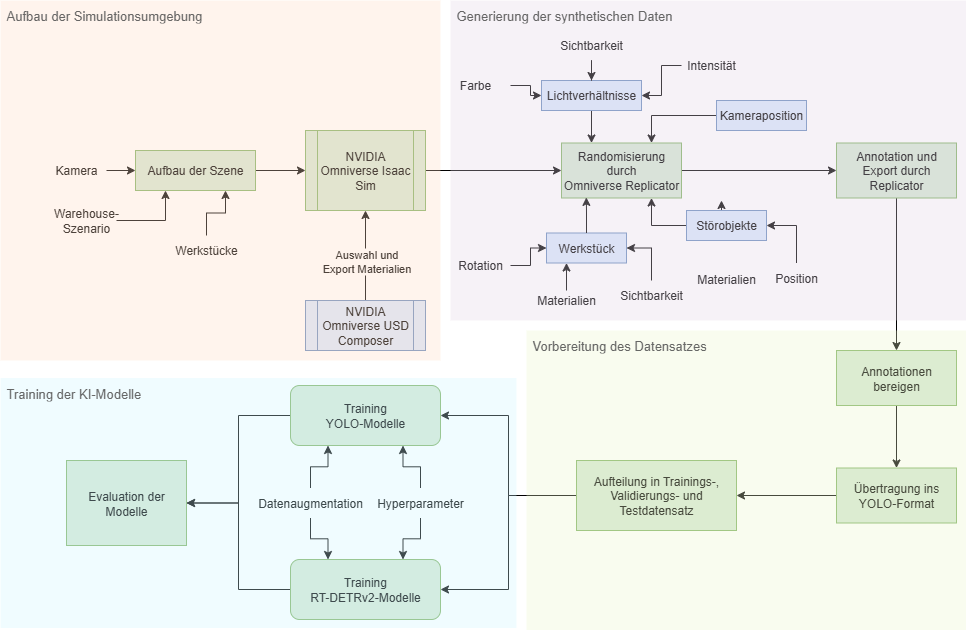
\includegraphics[width=0.9\linewidth]{graphics/Umsetzung_Diagramm.png}
    \caption{Grafische Visualisierung der Datengenerierungs- und Trainingspipeline}
    \label{fig:visualisierung_umsetzung}
\end{figure}

Abbildung \ref{fig:visualisierung_umsetzung} bietet eine grafische Übersicht über die in dieser Arbeit entwickelte Datengenerierungs- und Trainingspipeline.
Diese Pipeline wird im folgenden Kapitel detailliert beschrieben.

\section{Zielsetzung und Forschungsmethodik}
Ziel dieses Kapitels ist die praktische Umsetzung des in Kapitel \ref{sec:forschungsdesign} beschriebenen Forschungsdesigns. Der Fokus liegt auf der Realisierung einer Datenpipeline, mithilfe welcher automatisch synthetische Bilddaten inklusive deren Annotationen in einer Simulationsumgebung generiert werden. Die Pipeline soll so gestaltet sein, dass zentrale Parameter, die den Umfang und die Qualität der Daten betreffen, flexibel angepasst werden können. Darüber hinaus soll die Pipeline so konzipiert sein, dass sie leicht auf andere Fehlerfälle anpassbar ist, wodurch ihre Wiederverwendbarkeit und Übertragbarkeit auf andere Anwendungsszenarien sichergestellt wird. Die generierten Daten werden anschließend für das Training von \ac{KI}-Modellen aufbereitet. Darauf aufbauend erfolgt exemplarisch ein Training verschiedener Modelle und Modellarchitekturen zur Fehlererkennung, um die Qualität der durch die Pipeline erzeugten Daten zu validieren.

Methodisch folgt das Vorgehen dem \ac{DSR}-Paradigma, nach welchem das Artefakt in einem \textit{Build-and-Evaluate} Prozess entwickelt wird. Konkret wird das Artefakt in iterativen Zyklen entwickelt, getestet und verbessert. Dieses Kapitels konzentriert sich auf die Entwicklung des Artefakts, während eine detaillierte Evaluation der erzielten Ergebnisse in Kapitel \ref{chapter:Evaluation_Ergebnisse} folgt.


\section{Aufbau der Simulationsumgebung}

Im Sinne der Abbildung \ref{fig:visualisierung_umsetzung} wurden für die Umsetzung der Simulationsumgebung \textit{NVIDIA Omniverse}-Tools eingesetzt. Konkret kamen \textit{NVIDIA Omniverse USD Composer} auf Basis von \textit{Omniverse Kit} (Version 107.3.0) sowie \textit{NVIDIA Isaac Sim} (Version 4.5.0 rc.36) zum Einsatz. Diese Tools sind dafür bekannt, hochqualitative und realistische Bilddaten erzeugen zu können und wurden auch schon in ähnlichen Arbeiten, wie der Arbeit von \cite{monnet_investigating_2024} zur Generierung von Kratzern auf Metalloberflächen, verwendet.\footnote{Vgl. \cite[769 ff.]{monnet_investigating_2024}}

Der \textit{USD Composer} ist primär auf den Aufbau und die Gestaltung von \ac{CAD}-Szenen konzipiert\footcite{nvidia_omniverse_2025} und wurde in diesem Anwendungsfall hauptsächlich für die Auswahl und Speicherung unterschiedlicher Materialvarianten für das Werkstück und der Störobjekte verwendet. Der Großteil der Umsetzung erfolgte allerdings in \textit{Isaac Sim}\footcite{nvidia_isaac_2025}, da dort die Implementierung des \textit{Omniverse Replicator} eine effiziente Realisierung der \textit{Domain Randomization} sowie den Export der generierten Bilddaten ermöglichte.\footcite{nvidia_replicator_2025}

Als Grundlage der Simulationsumgebung diente ein von \textit{Isaac Sim} bereitgestelltes Warehouse-Szenario, welches aufgrund der bereits implementierten Beleuchtungselementen ausgewählt wurde. Hierdurch kann eine realitätsnahe Umsetzung, insbesondere in Hinblick auf die Lichtverhältnisse, erreicht werden. In die Szene wurde außerdem eine von TRUMPF bereitgestellte Fertigungsmaschine platziert sowie ergänzend 84 Zustände eines Blechs im Schneideprozess, einschließlich der vollständig ausgeschnittenen Teile. Die CAD-Dateien für Blech und Maschine wurden aus der Software \textit{Siemens NX} im USD-Format exportiert. Grundsätzlich können jedoch jegliche USD-Modelle eingebunden werden, wodurch die Simulationsumgebung flexibel erweiterbar bleibt. 

Zur Bildaufnahme wurde eine virtuelle Kamera implementiert, welche ebenfalls durch \textit{Isaac Sim} bereitgestellt wird. Diese wurde mit Parametern konfiguriert, die den realen Produktionskameras entsprechen, wodurch eine möglichst enge Annäherung an reale Produktionsszenarien erreicht werden kann.


\section{Generierung der synthetischen Bilddaten}

Aufbauend auf der in Abbildung \ref{fig:visualisierung_umsetzung} dargestellten Systematik erfolgte im Anschluss an den Aufbau der Simulationsumgebung die Generierung der Bilddaten mit zufälliger Variation zentraler Parameter im Sinne der \textit{Domain Randomization} mithilfe des \textit{Omniverse Replicator}.\footcite{nvidia_replicator_2025}
Bei dem \textit{Omniverse Replicator} handelt es sich um ein Framework, mithilfe welchem Pipelines zur Generierung umfassender synthetischer Daten gebaut werden können. Durch diesen ist es möglich, bestehende USD-Szenen zu Nutzen oder neue Szenen dynamisch aufzubauen. Verschiedene Elemente und deren Eigenschaften in der Szene können mit diesem Tool zufällig variiert, automatisch annotiert und exportiert werden.\footnote{Vgl. \cite{nvidia_replicator_2025}}

Aufgrund zeitlicher Beschränkungen wurde exemplarisch ein konkreter Anwendungsfall umgesetzt, der wie folgt definiert ist:
Ein vollständig ausgeschnittenes Blech wird auf der Maschine platziert und die ausgeschnittenen Teile für jedes Bild zufällig in die vorgesehen Aussparung zurück platziert. Die Teile werden dabei zufällig um einen Winkel rotiert, wessen Spannweite durch einen Parameter in der Pipeline festgelegt werden kann. In diesem Anwendungsfall betrug der Rotationsbereich -4° bis +4° relativ zur Ausgangsposition. Weitere potenzielle Szenarien, wie beispielsweise verschobenen oder nicht vollständig herausgetrennte Teile, konnten aufgrund zeitlicher Einschränkungen nicht mehr implementiert werden, können jedoch aufgrund der flexiblen Architektur problemlos ergänzt werden.

Neben der Variation der Werkstücke wurden auch Umgebungsparameter randomisiert. Dazu zählen insbesondere die Materialien des Blechs und der ausgeschnittenen Teile sowie die Umgebungsbeleuchtung. Bei letzterer wurde sowohl die Sichtbarkeit einzelner Lichter als auch deren Intensität und Farbe zufällig variiert. Zudem wurde die Position der Kamera randomisiert, wobei sowohl die Entfernung zum Werkstück, als auch die horizontale und vertikale Position innerhalb vorgegebener Grenzen variiert wurde. Auf diese Weise sollte die Robustheit des Modells gegenüber unterschiedlicher Blickwinkel und Bildausschnitte erhöht werden.

Zentrale Parameter der Pipeline können zu Beginn des Skripts nach Bedarf angepasst werden. Hierzu zählen verschiedene  Einstellungen zur Bildqualität, wie beispielsweise Antialiasing, Bildauflösung und Parameter zur Simulation des Lichts. Auch die Konfiguration der \textit{Domain Randomization} kann im Skript angepasst werden. Die konkrete Implementierung der Datengenerierungspipeline ist in Anhang \ref{anhang:replicator_code} aufgeführt.\footnote{Vgl. Anhang \ref{anhang:replicator_code}}

\begin{figure}[htb]
    \centering
    \begin{subfigure}{0.49\textwidth}
        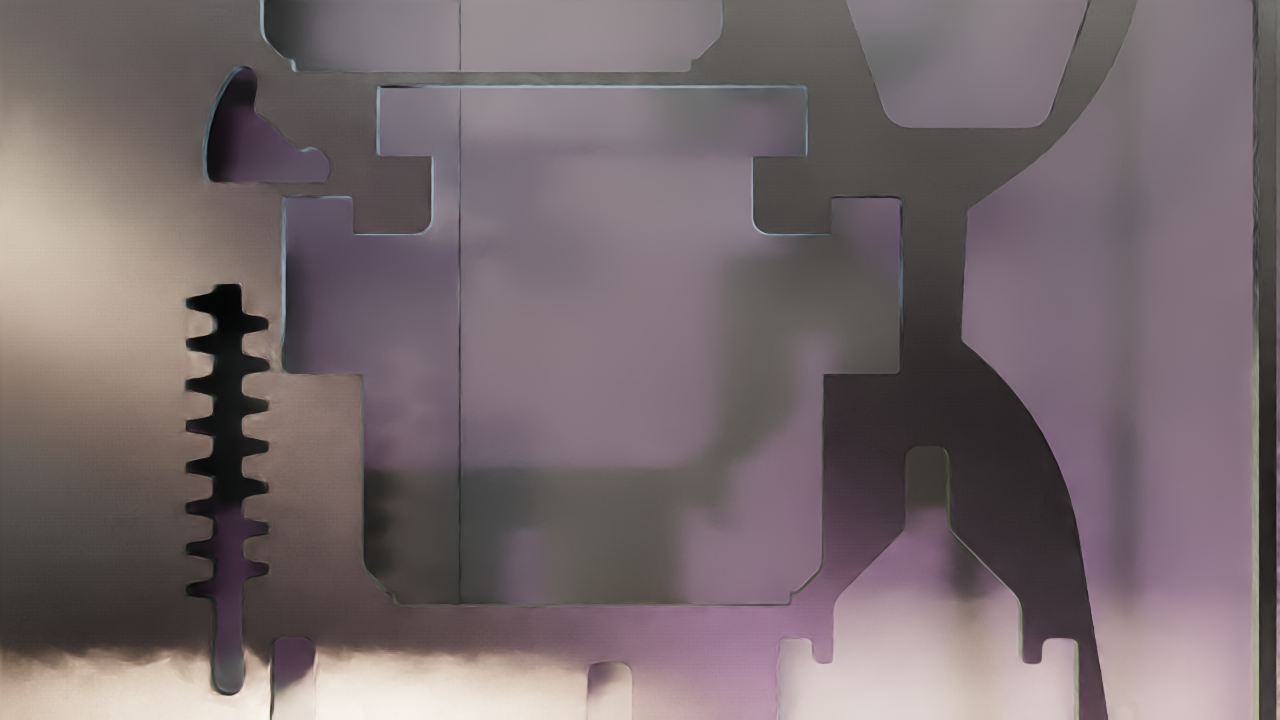
\includegraphics[width=\textwidth]{graphics/example_synthetic_images/Beispiel_Replicator_1.png}
    \end{subfigure}
    \hfill
    \begin{subfigure}{0.49\textwidth}
        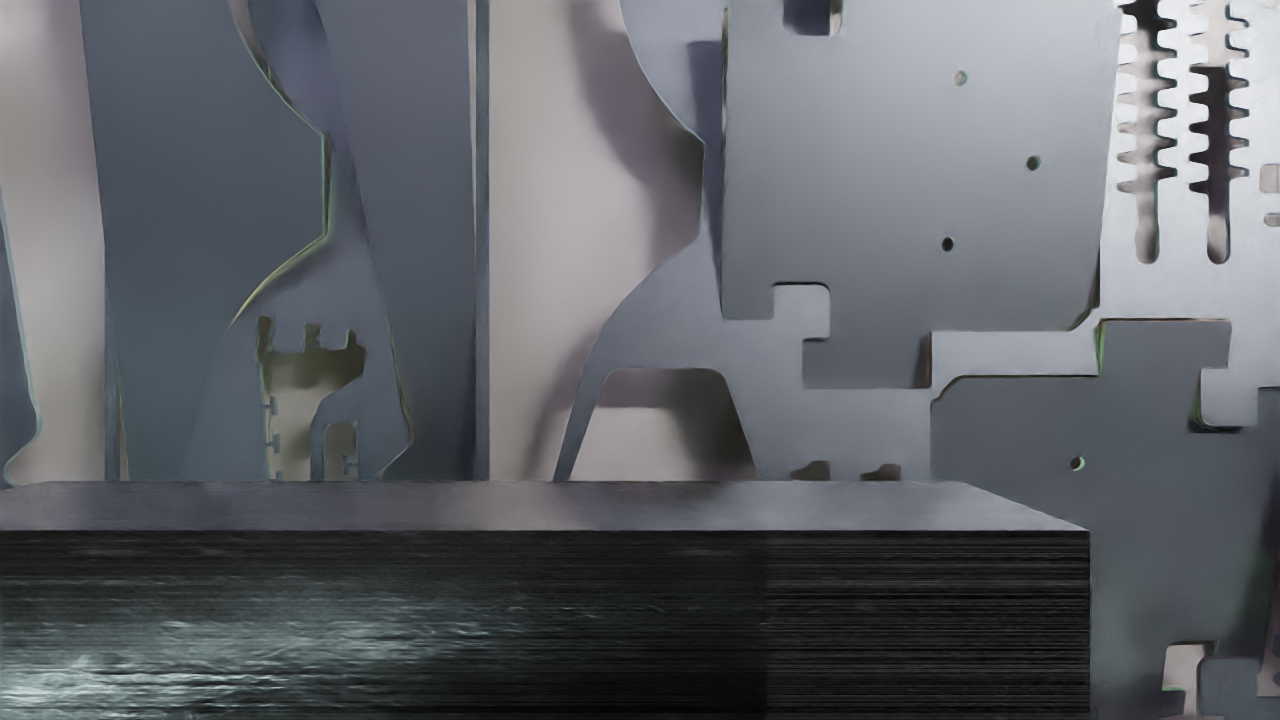
\includegraphics[width=\textwidth]{graphics/example_synthetic_images/Beispiel_Replicator_2.png}
    \end{subfigure}
    \caption{Beispiele für exportierte Bilder aus dem Replicator}
    \label{fig:beispiel_replicator}
\end{figure}

Abbildung \ref{fig:beispiel_replicator} zeigt zwei beispielhafte Bilder, welche mithilfe des Replicators generiert wurden. Insgesamt wurden 1077 Bilder exportiert. Ein größerer Umfang wäre prinzipiell möglich gewesen, war jedoch aufgrund der verfügbaren Rechenleistung und des damit verbundenen Zeitaufwands im Rahmen dieser Arbeit nicht umsetzbar. 

Diese Bilddaten werden dabei durch den Replicator automatisch annotiert. Ein Beispiel hierfür ist in Abbildung \ref{fig:replicator_annotationen} dargestellt. Zwar liegen die exportierten Annotationen im Textformat vor, für dieses Beispiel wurden sie jedoch zur Veranschaulichung visualisiert.

\begin{figure}[htb]
    \centering
    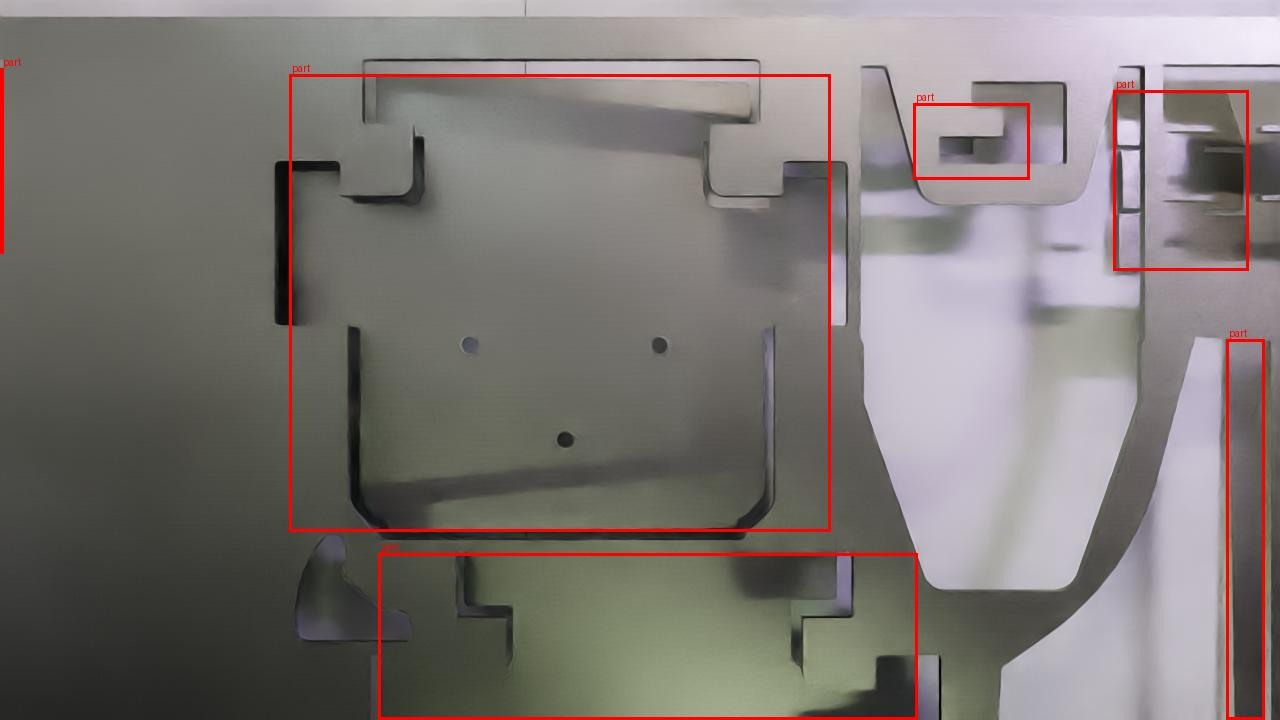
\includegraphics[width=0.9\linewidth]{graphics/example_synthetic_images/Beispiel_Annotation.jpg}
    \caption{Beispiel einer durch den Replicator automatisch erzeugten Annotation (grafisch visualisiert)}
    \label{fig:replicator_annotationen}
\end{figure}


\section[Training von KI-Modellen auf synthetischen Bilddaten]{Training von \ac{KI}-Modellen auf synthetischen Bilddaten}

\subsection{Auswahl der KI Architekturen und Modelle}
Als erstes Modell wurde die \ac{YOLO}-Architektur ausgewählt, welche auf \acp{CNN} basiert und sich in zahlreichen Benchmarks als leistungsfähiger und effizienter Standard im Bereich der Objekterkennung erwiesen hat. \footnote{Vgl. \cite[771]{monnet_investigating_2024}; \cite{bilous_comparison_2024}}
Verwendet wurde dabei die Implementierung von \textit{Ultralytics}, die aufgrund ihrer einfachen Handhabung, umfangreicher Dokumentation und integrierter Möglichkeiten zur Datenaugmentation ein besonders praxistaugliches Framework bietet.\footnote{Vgl. \cite{yolo11_ultralytics}}
Aufgrund begrenzter Hardwarekapazitäten konzentrierte sich diese Arbeit auf das Training kleinerer Modellvarianten (Nano, Small und Medium).

Angesichts der kleinen Größe des Datensatzes und der Handhabung von synthetischen Daten wurde ein relativ hoher Grad an Datenaugmentation beim Training eingesetzt, um die Generalisierungsfähigkeit der Modelle zu verbessern.

\subsection{Vorbereitung des Datensatzes und Training der Modelle}
Vor dem tatsächlichen Training der \ac{KI}-Modelle wurden die durch den \textit{Omniverse Replicator} exportierten Bild- und Annotationsdaten im Sinne der Abbildung \ref{fig:visualisierung_umsetzung} zuerst in ein geeignetes Format überführt. Der Export aus dem Replicator erfolgte im sogenannten KITTI-Format, welches sich nicht unmittelbar für die nachfolgenden Trainingspipelines eignete. Für das Training der \ac{YOLO} Modelle mussten die Annotationsdaten in das \ac{YOLO}-Format konvertiert werden. Dazu wurden Bild- und Annotationsdateien in einer automatisierten Pipeline konsolidiert, das Format der Annotationsdaten angepasst und der Datensatz in Trainings-, Validierungs- und Test-Splits unterteilt.\footnote{Vgl. Anhang  \ref{anhang:datensatz_erstellen_code}} Dabei wurde ein Split von 70/20/10 (70\% Training, 20\% Validierung, 10\% Test) gewählt, was eine anerkannte Aufteilung in der Literatur darstellt.\footnote{Vgl. 
\cite[261]{urgo_monitoring_2024}; \cite[3]{griem_synthetic_2025}; \cite[5]{khirodkar_domain_2018}}

Auf diesem Datensatz wurden drei Modelle der YOLO11-Architektur trainiert (Nano, Small und Medium). Um die effektive Größe und Varianz des Trainingsdatensatzes zu erhöhen, kamen umfangreiche Verfahren der Datenaugmentation zum Einsatz, welche durch das Trainingsframework von \textit{Ultralytics} bereitgestellt werden.\footnote{Vgl. Anhang \ref{anhang:yolo_code}} Die Auswahl der Hyperparameter bestimmte sich primär aus der offiziellen Dokumentation von \textit{Ultralytics}\footnote{Vgl. \cite{ultralytics_hyperparameter-optimierung_nodate}; \cite{ultralytics_yolo-datenerweiterung_nodate}} sowie einem iterativen Trainingsansatz.\footnote{ChatGPT-5 wurde unterstützend bei der Optimierung der Hyperparameter eingesetzt.} Die Anzahl der Epochen wurde auf 200 festgelegt, mit dem Ziel, durch eine hohe Augmentierung in Kombination mit einer hohen Anzahl an Epochen den kleinen Datensatz bestmöglich auszunutzen und \textit{Overfitting} zu vermeiden.

Neben den \ac{YOLO}-Modellen wurde ergänzend ein transformerbasiertes Modell trainiert. Da herkömmliche Transformer-Architekturen bei kleinen Datensätzen ineffizient sind, wurde der \ac{RT-DETR}v2 gewählt, eine speziell optimierte Variante für ressourcenschonendes Training \footnote{Vgl. \cite{zhao_detrs_2023}}.
Hier wurde sowohl ein Modell mit Datenaugmentation als auch eines ohne Datenaugmentation trainiert. Aus zeitlichen Gründen wurde hierbei ausschließlich eine kleinere Variante (\ac{RT-DETR}-18) eingesetzt.\footnote{Vgl. Anhang \ref{anhang:rt_detr_code}} Auch hier wurde eine hohe Anzahl an Epochen (220) gewählt, um den kleinen Datensatz bestmöglich auszuschöpfen. Allerdings konvergierten beide Modelle bereits nach kurzer Zeit und beendeten das Training bereits nach etwa 40 Epochen, da keine weiteren Verbesserungen erzielt werden konnten.

\subsection{Probleme während des Trainings}
Im Rahmen der Evaluation traten spezifische Probleme im Datenpipeline-Design auf. So zeigte sich, dass die mit dem KITTI-Writer erzeugten Bounding Boxes fehlerhaft erzeugt wurden, wodurch mehr Annotationen als tatsächlich Objekte vorhanden waren. Dies hatte zur Folge, dass Bounding Boxes nicht mit den tatsächlichen Objektpositionen übereinstimmten, was eine Bereinigung der Annotationsdaten erforderlich machte. Zudem wurden teilweise Bild-Label-Paare doppelt in verschiedenen Datensplits abgelegt (\textit{Data Leakage}), was zu einer Überschätzung der Modellleistung in der Validierung führte. Diese Inkonsistenzen wurden behoben und die Trainingsläufe wiederholt.


\subsection[Evaluation der KI-Modelle]{Evaluation der \ac{KI}-Modelle}\label{subsec:umsetzung_evaluation_modelle}
Die trainierten Modelle wurden zunächst auf dem zuvor definierten Test-Split des synthetischen Datensatzes evaluiert.\footnote{Vgl. Anhang \ref{anhang:evaluation_yolo_code} und Anhang \ref{anhang:evaluation_rtdetr_code}} Anhand der in Abschnitt \ref{subsec:evaluationsdesign} beschriebenen Metriken konnte so eine erste Einschätzung der Modellleistung erfolgen. Bei unzureichenden Ergebnissen wurden Trainingsparameter angepasst und das Training erneut durchgeführt. Durch diesen iterativen Prozess konnte die Modellleistung auf synthetischen Daten stetig verbessert werden.

Wie bereits in Abschnitt \ref{subsec:evaluationsdesign} beschrieben, wurden die Modellvorhersagen vor der Berechnung der Metriken einem \ac{NMS} unterzogen. Hierbei wurde eine \ac{IoU}-Schwelle von 0.5 verwendet, welches ein üblicher Wert in der Praxis darstellt.\footnote{Vgl. \cite[8]{he_mask_2017}; \cite[3]{bodla_soft-nms_2017}} Überlappende Bounding Boxes mit einem Überschneidungsgrad von 50\% werden dementsprechend durch \ac{NMS} reduziert.

Um die Generalisierungsfähigkeit der Modelle und ihre Übertragbarkeit auf reale Anwendungsfaälle zu überprüfen, wurde die Modellleistung ergänzend auf realen Bildern evaluiert.\footnote{Vgl. Anhang \ref{anhang:evaluation_yolo_code} und Anhang \ref{anhang:evaluation_rtdetr_code}} Dazu wurde aus \textit{TRUMPF Visual Insights}, einer unternehmensinternen Software, in welcher Videos der Produktionsmaschinen bei Fehlerfällen gespeichert sind, 34 Bilder gesammelt, welche dem simulierten Fehlerfall ähnelten. Diese Bilder wurden manuell annotiert und dienten als unabhängiger Referenzdatensatz zur abschließenden Evaluation der Modelle. Bei unzureichender Leistung wurde auch hier das Training mit angepassten Parametern wiederholt, wobei die Anzahl an Iterationen aufgrund zeitlicher Limitationen eingeschränkt war.




\chapter[Evaluation der KI-Modelle zur Fehlererkennung bei Werkzeugmaschinen]{Evaluation der \ac{KI}-Modelle zur Fehlererkennung bei Werkzeugmaschinen \footnote{Sprachlich geglättet durch ChatGPT-5}}
\label{chapter:Evaluation_Ergebnisse}

\section{Zielsetzung und Forschungsmethodik}
Ziel der Evaluation ist, die Leistungsfähigkeit der auf synthetischen Daten trainierten \ac{KI}-Modelle zur Erkennung von Fehlerfällen bei Werkzeugmaschinen zu überprüfen. Dabei wird sowohl die Leistung der KI-Modelle auf synthetischen Daten als auch der Übertrag auf die Realität durch Tests auf realen Daten betrachtet. Dies schafft eine Basis, auf welcher die Eignung synthetischer Daten für Anwendungszwecke solcher Art diskutiert werden kann.

Methodisch orientiert sich die Evaluation am im Kapitel \ref{subsec:evaluationsdesign} dargestellten Design. Zunächst werden die Modelle auf dem Test-Split des synthetischen Datensatzes evaluiert, um einen ersten Eindruck der Leistungs- und Generalisierungsfähigkeit zu erlangen. Gleichzeitig dient dieser Schritt der Validierung der Pipeline zur Datengenerierung, da hierdurch Konsistenz und Eignung synthetischer Bilddaten für das Training von \ac{KI}-Modellen untersucht werden kann.

Ergänzend erfolgt eine Evaluation auf einem realen Testdatensatz aus 34 Bildern, welcher wie in Kapitel \ref{subsec:umsetzung_evaluation_modelle} beschrieben zusammengestellt und annotiert wurde. Diese Untersuchung dient primär der Analyse der Eignung von auf synthetischen Daten trainierten Modellen in realen Anwendungsumgebungen sowie der Betrachtung des Einflusses des \textit{Domain Gaps}. Auf dieser Grundlage lässt sich auch der Bedarf an zukünftiger Forschung in diesem Themengebiet ableiten.


\subsection[Evaluation der YOLO-Modelle]{Evaluation der \ac{YOLO}-Modelle}

Zuerst wurden die drei \ac{YOLO}-Modelle auf dem synthetischen Datensatz evaluiert. Der Verlauf zentraler Metriken während des Trainings ist exemplarisch für das \ac{YOLO}-Medium Modell in Abbildung \ref{fig:training_verlauf} dargestellt. Es ist zu erkennen, dass die Modelle bereits nach wenigen Epochen eine gute Leistung auf dem Validierungsdatensatz erzielen konnten und schlussendlich eine Konvergenz zu erkennen ist. Ein ähnlicher Verlauf zeigte sich auch bei den beiden anderen Modellvarianten.\footnote{Vgl. Anhang \ref{anhang:training_verlauf}}

\begin{figure}[htb]
      \centering                        
      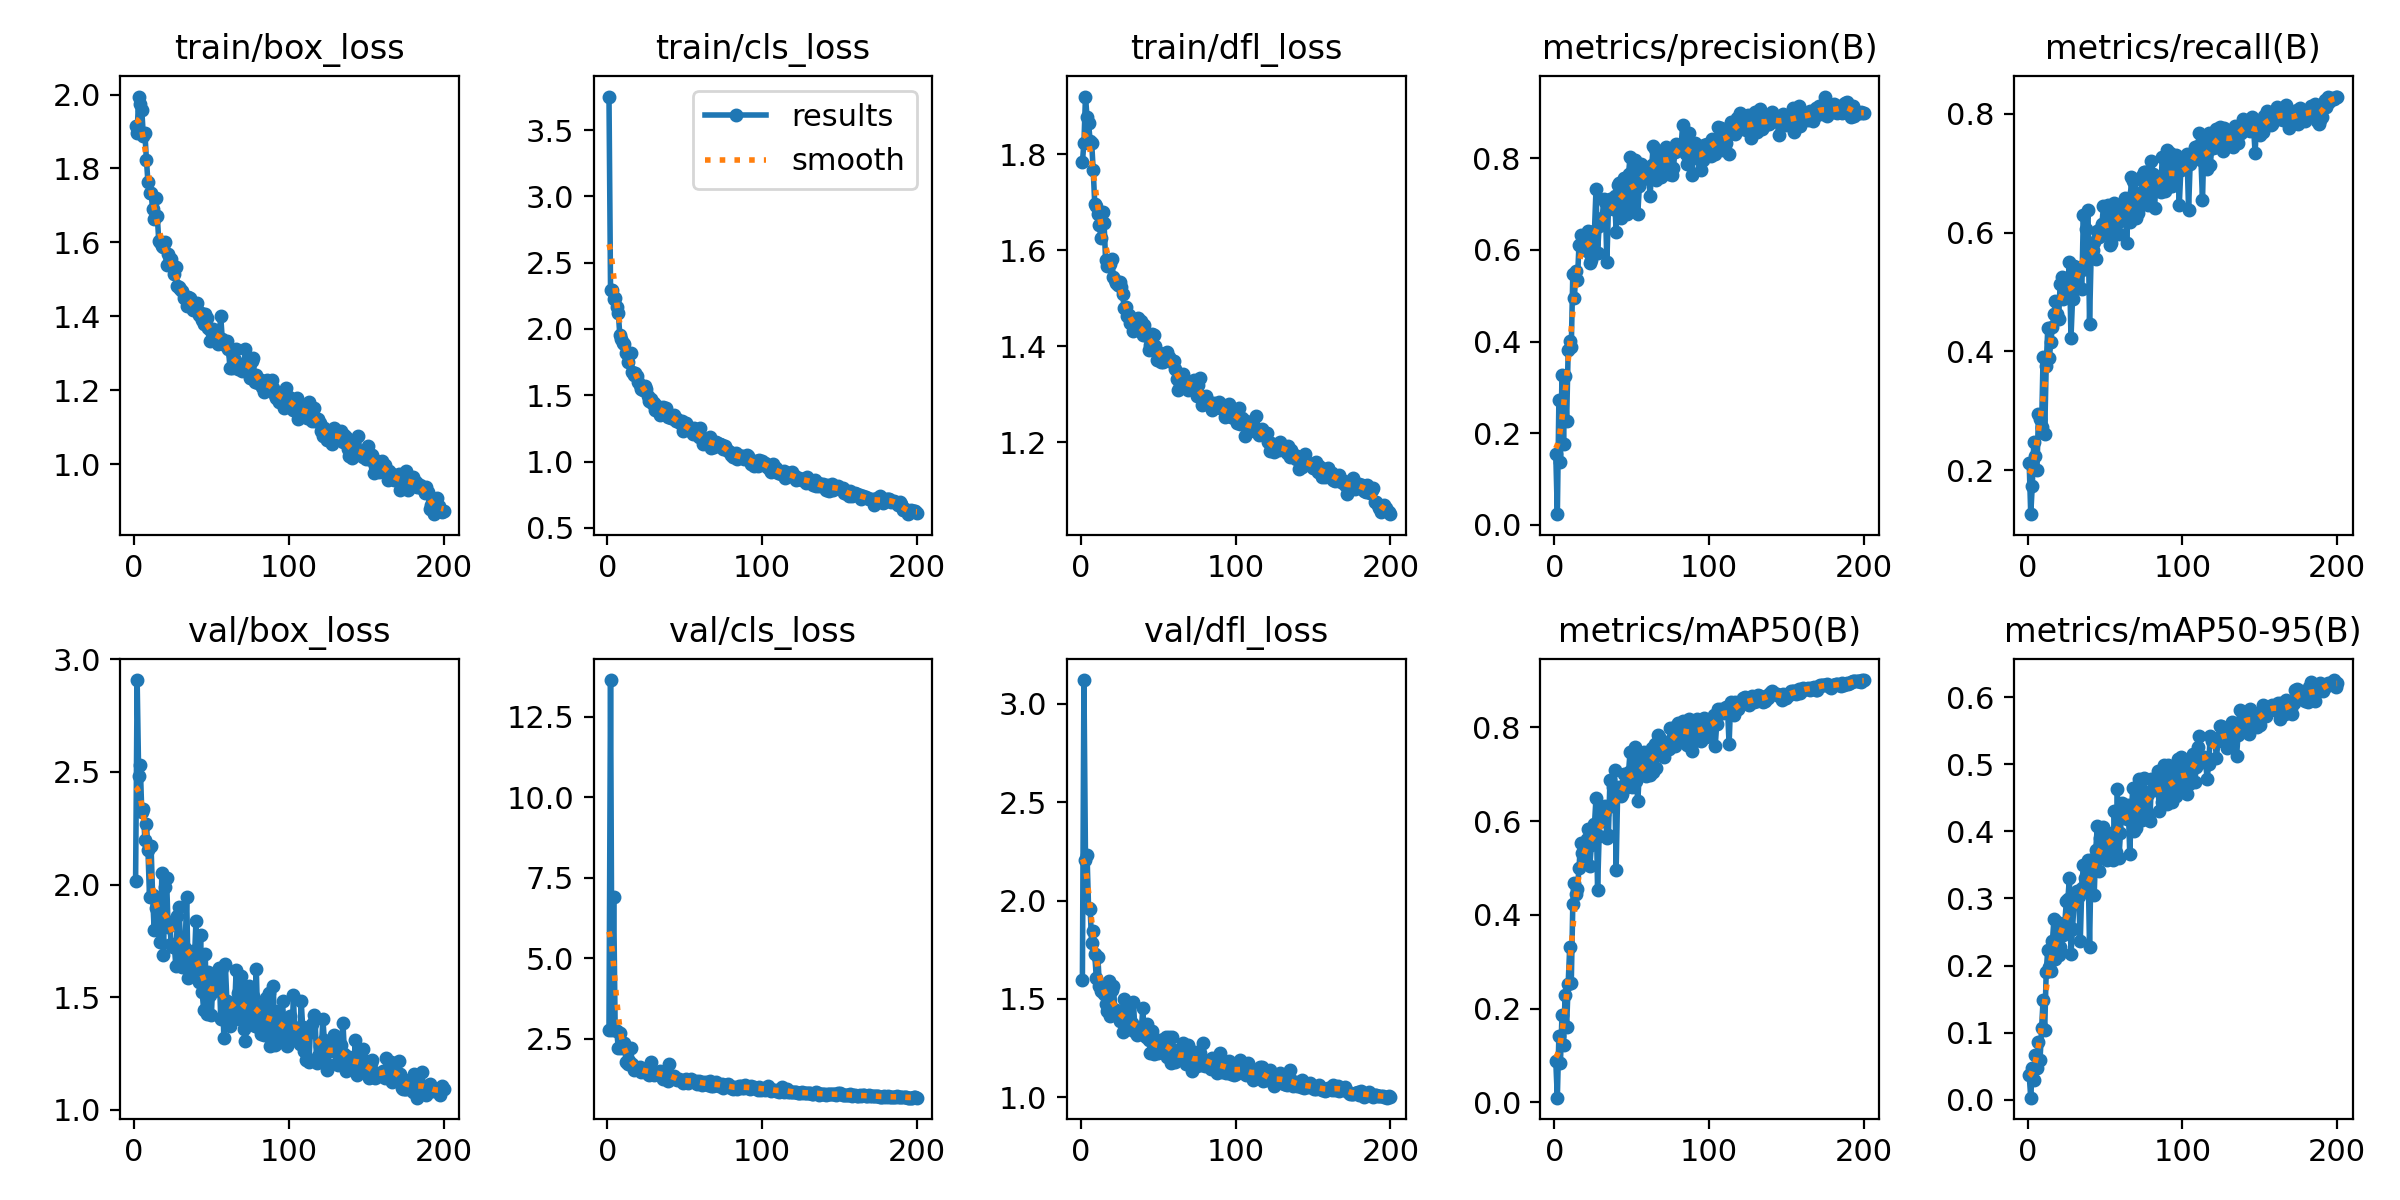
\includegraphics[width=0.9\linewidth]{graphics/yolo_eval/model_m/results.png}
      \caption{Trainingsverlauf des \ac{YOLO}-Modells Medium}
      \label{fig:training_verlauf}
\end{figure}

Wie in Tabelle \ref{tab:yolo_results} dargestellt, zeigten alle drei Modelle eine konsistente Leistung auf dem synthetischen Test-Split. Das \ac{YOLO}-Small Modell erzielte dabei die beste Leistung mit einer \ac{mAP}@50 von 0.9080 und einer \ac{mAP}@[.5:.95] von 0.6605. Auch beim Sensitivität Wert erreichte dieses Modell mit 0.8094 den höchsten Wert. Bei allen drei Modellen lag die Präzision über 0.9, was auf eine geringe Rate an \ac{FP} hinweist.  Es ist jedoch zu beachten, dass alle Modelle bei allen Metriken nahe beieinander liegen und keine signifikanten Unterschiede zwischen dem kleinsten und dem größten Modell erkennbar waren. 

Abbildung \ref{fig:pr_kurven} zeigt ergänzend die Präzisions-Sensitivitäts-Kurven des größten und kleinsten trainierten Modells. Beide Kurven zeigen einen ähnlichen Verlauf, wobei das \ac{YOLO}-Medium Modell etwas höhere Präzisions-Werte bei höherer Sensitivät erreichte. Insgesamt zeigen alle Modelle jedoch keine signifikanten Unterschiede,\footnote{Vgl. Anhang \ref{anhang:pr_curve_small}}sondern vergleichbar gute Ergebnisse auch bei hohen Sensitivitätswerten. 
Zusammenfassend lässt sich festhalten, dass alle drei Modelle auf dem synthetischen Datensatz eine gute Leistung erbringen konnten, was die Konsistenz und Eignung der mittels der Pipeline generierten synthetischen Daten für das Training von \ac{KI}-Modellen unterstreicht.

\begin{figure}[htb]
    \centering
    \begin{subfigure}{0.49\textwidth}
        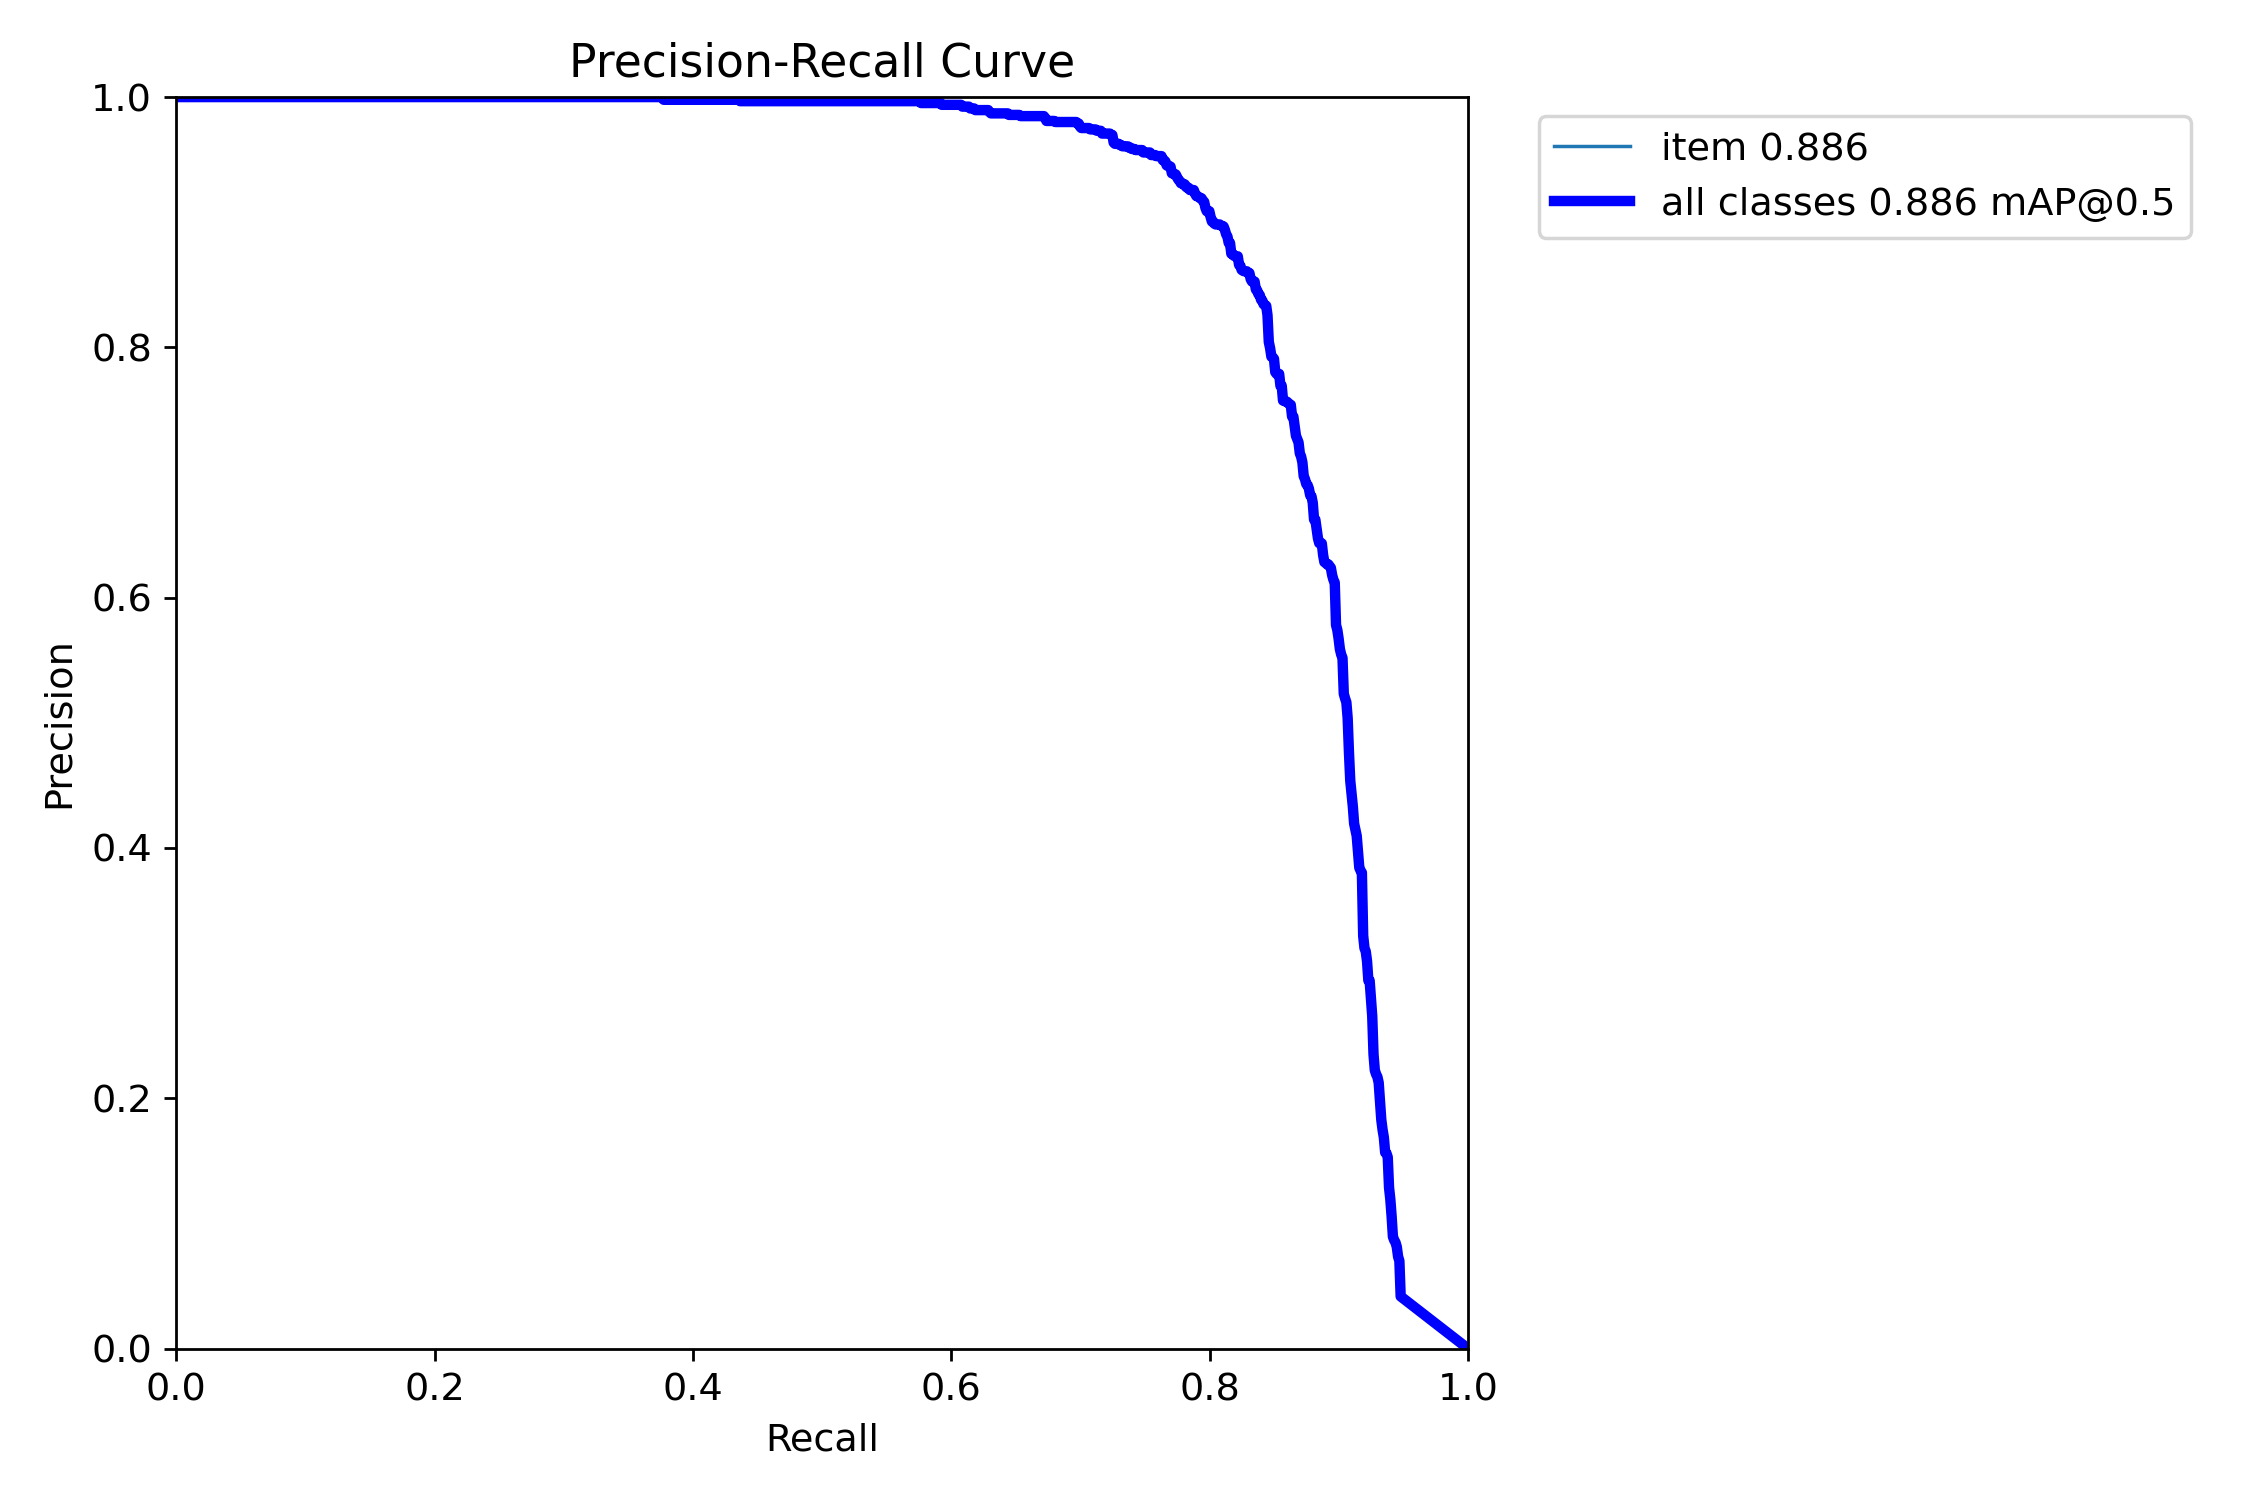
\includegraphics[width=\textwidth]{graphics/yolo_eval/model_n/BoxPR_curve.png}
        \caption{\ac{YOLO} Modell Nano}
    \end{subfigure}
    \hfill
    \begin{subfigure}{0.49\textwidth}
        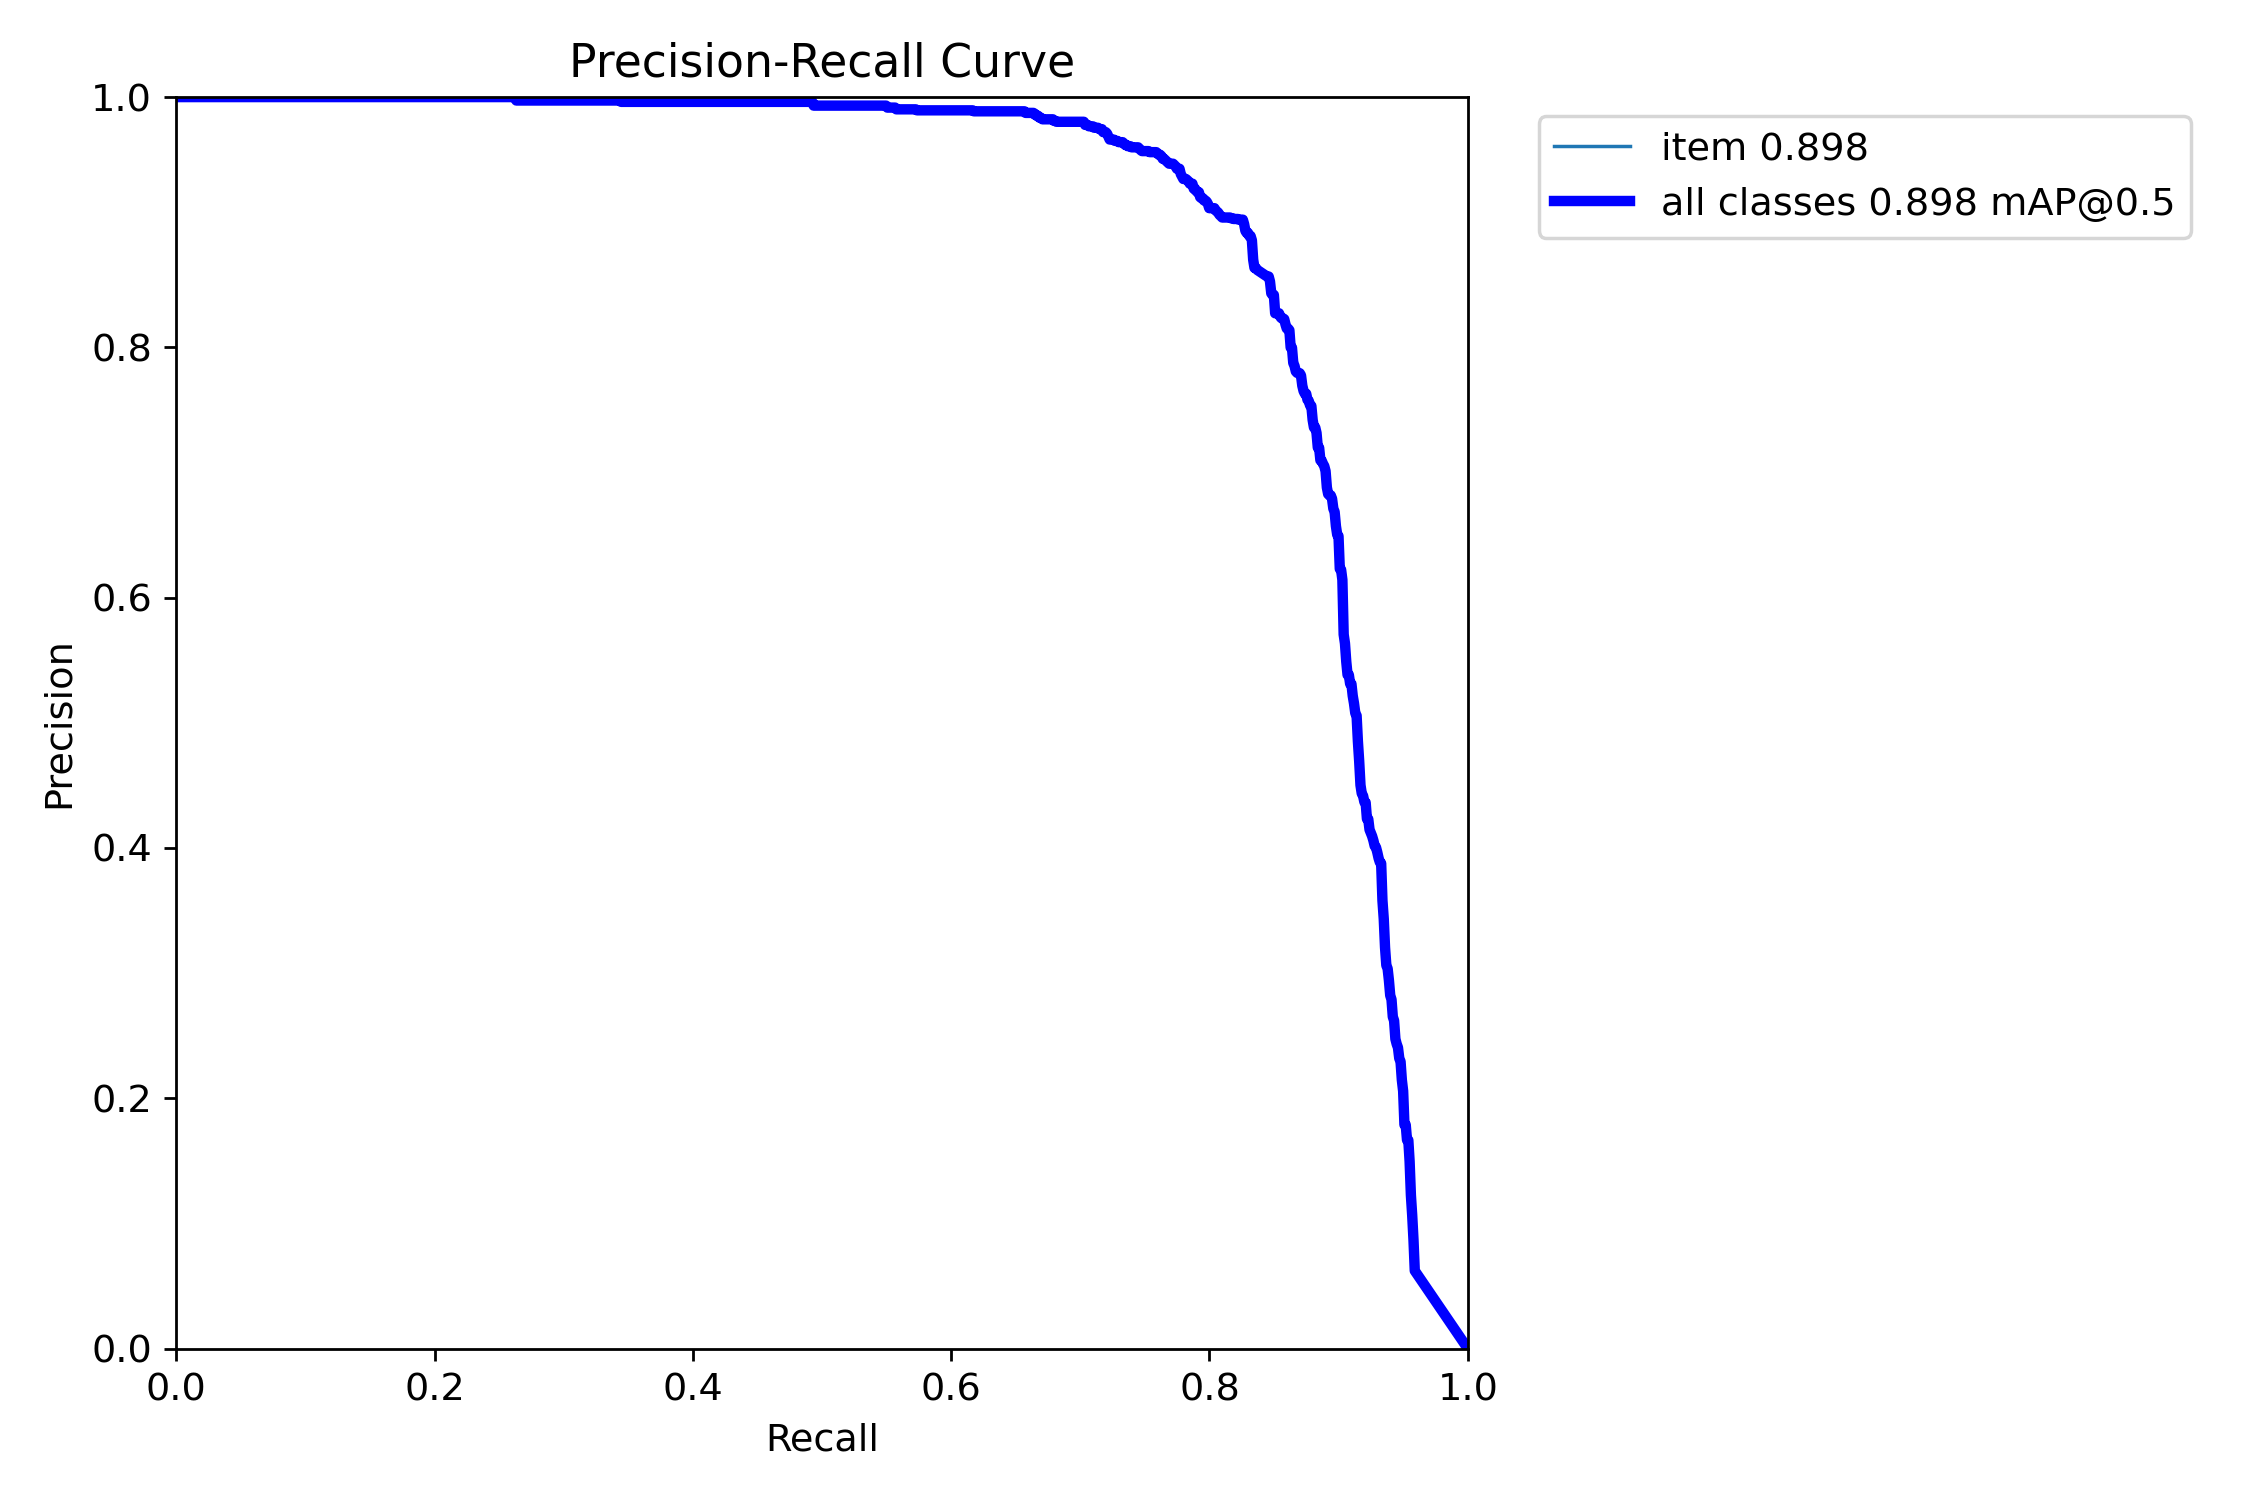
\includegraphics[width=\textwidth]{graphics/yolo_eval/model_m/BoxPR_curve.png}
        \caption{\ac{YOLO} Modell Medium}
    \end{subfigure}
    \caption{Präzision-Sensitivität-Kurven der \ac{YOLO}-Modelle Nano und Medium}
    \label{fig:pr_kurven}
\end{figure}


Auf dem realen Datensatz hingegen zeigten alle drei \ac{YOLO}-Modelle eine deutlich reduzierte Leistung. Das \ac{YOLO}-Medium-Modell erzielte mit einer \ac{mAP}@50 von 0.0712 die beste Leistung, kann jedoch mit der erbrachten Leistung nicht als zufriedenstellend angesehen werden. Die anderen beiden Modelle wiesen einen noch stärkeren Leistungsabfall auf. Alle Modelle hatten hier deutlich geringe Präzisions- und Sensitivität-Werte, was auf eine höhere Anzahl an \ac{FP} und \ac{FN} schließen lässt. Dies verdeutlicht den Einfluss des \textit{Domain Gaps}, da die Modelle, obwohl sie auf synthetischen Daten gute Ergebnisse lieferten, Schwierigkeiten hatten, ihre Leistung auf reale Anwendungsfälle zu übertragen und zeigten aufgrund der geringen Anzahl an \ac{TP} keine Konsistenz in der korrekten Erkennung von Fehlerfällen.

\begin{table}[htb]
\centering
    \resizebox{\textwidth}{!}{
    \begin{tabular}{||c c c c c c c||} 
        \hline
        Modell & Datensatz & Augmentierung & mAP@50 & mAP@[.5:.95] & Präzision & Sensitivität \\ [0.5ex] 
        \hline\hline
        YOLO-n & synthetisch & ja & 0.8872 & 0.6628 & 0.9368 & 0.7510 \\ 
        \hline
        YOLO-s & synthetisch & ja & 0.9176 & 0.6673 & 0.9156 & 0.8250 \\
        \hline
        YOLO-m & synthetisch & ja & 0.8957 & 0.6607 & 0.9153 & 0.7996 \\ 
        \hline
        RT-DETR-v2-r18 & synthetisch & ja & 0.2790 & 0.1892 & 0.1966 & 0.6335 \\ 
        \hline
        RT-DETR-v2-r18 & synthetisch & nein & 0.5160 & 0.3913 & 0.1634 & 0.8070 \\ 
        
        \hline\hline
        
        YOLO-n & real & ja & 0.0161 & 0.0062 & 0.0425 & 0.0667 \\ 
        \hline
        YOLO-s & real & ja & 0.0115 & 0.0028 & 0.0240 & 0.1000 \\
        \hline
        YOLO-m & real & ja & 0.0712 & 0.0402 & 0.1087 & 0.1000 \\
        \hline
        RT-DETR-v2-r18 & real & ja & 0.0050 & 0.0020 & 0.0066 & 0.4000 \\ 
        \hline
        RT-DETR-v2-r18 & real & nein & 0.0052 & 0.0016 & 0.0066 & 0.4667 \\ 
        \hline
    \end{tabular}
    }
\caption{Ergebnisse zentraler Metriken der \ac{KI}-Modelle mit \textit{Confidence Threshold 0.1}}
\label{tab:yolo_results}
\end{table}


\subsection[Evaluation des RT-DETR Modells]{Evaluation des \ac{RT-DETR} Modells}

Betrachtet man die Ergebnisse der beiden \ac{RT-DETR}-r18-Modelle, so zeigt sich ein deutlich anderes Bild als bei den \ac{YOLO}-Modellen. Trotz der schnellen Konvergenz erzielten beide Modelle bereits auf dem synthetischen Test-Split eine signifkant schlechtere Leistung als alle drei \ac{CNN}-basierten Modelle. Auffällig ist dabei, dass die bessere Leistung das Modell, welches ohne Datenaugmentierung trainiert wurde, erzielen konnte. Dieses erreichte jedoch dennoch nur eine \ac{mAP}@50 von 0.5160 und eine \ac{mAP}@[.5:.95] von 0.3913. Besonders auffällig sind die sehr niedrigen Präzisions-Werte bei beiden Trainingsansätzen, was auf eine hohe Rate an \ac{FP} hinweist, während beim Sensitivität mit 0.8070 beim Training ohne Datenaugmentation ein vergleichsweiser akzeptabler Wert erreicht werden konnten. Dies deutet darauf hin, dass das Modell zwar einige der tatsächlichen Fehlerfälle erkennt, jedoch auch viele \ac{FP} generiert. Angesichts dieser hohen Zahl an \ac{FP} ist keine Konsistenz in der korrekten Erkennung ersichtlich und es könnte sich auch um zufällige Treffer handeln.

Bei der Evaluation auf dem realen Datensatz verschlechterte sich die Leistung beider Modelle weiter. Mit \ac{mAP}@50 und \ac{mAP}@[.5:.95] Werten nahe 0 zeigten die Modelle eine nahezu unbrauchbare Leistung. Sowohl Präzisions als auch Senstivitäts-Werte fielen im Vergleich zu dem synthetischen Datensatz nochmals deutlich ab. Daraus ist abzuleiten, dass die Modelle zwar viele Elemente des Bildes als Fehler klassifizieren, jedoch kaum korrekte Vorhersagen treffen und tatsächliche Fehler übersehen. Betrachtet man die in Abbildung \ref{fig:beispiel_vorhersage_rtdetr} dargestellte visualisierte Vorhersage des Modells mit Datenaugmentierung, wird dieser Verdacht bestätigt. Es sind zahlreiche \textit{Bounding Boxes} zu erkennen, welche jedoch kaum mit den tatsächlichen Fehlern übereinstimmen. Damit kann zusammengefasst werden, dass die \ac{RT-DETR}-Modelle sowohl auf synthetischen als auch auf realen Daten eine deutlich schlechtere Leistung erbrachten als die \ac{YOLO}-Modelle und auf keinem der Datensätze eine zufriendenstellende Leistung aufweisen konnten.

\begin{figure}[htb]
      \centering                        
      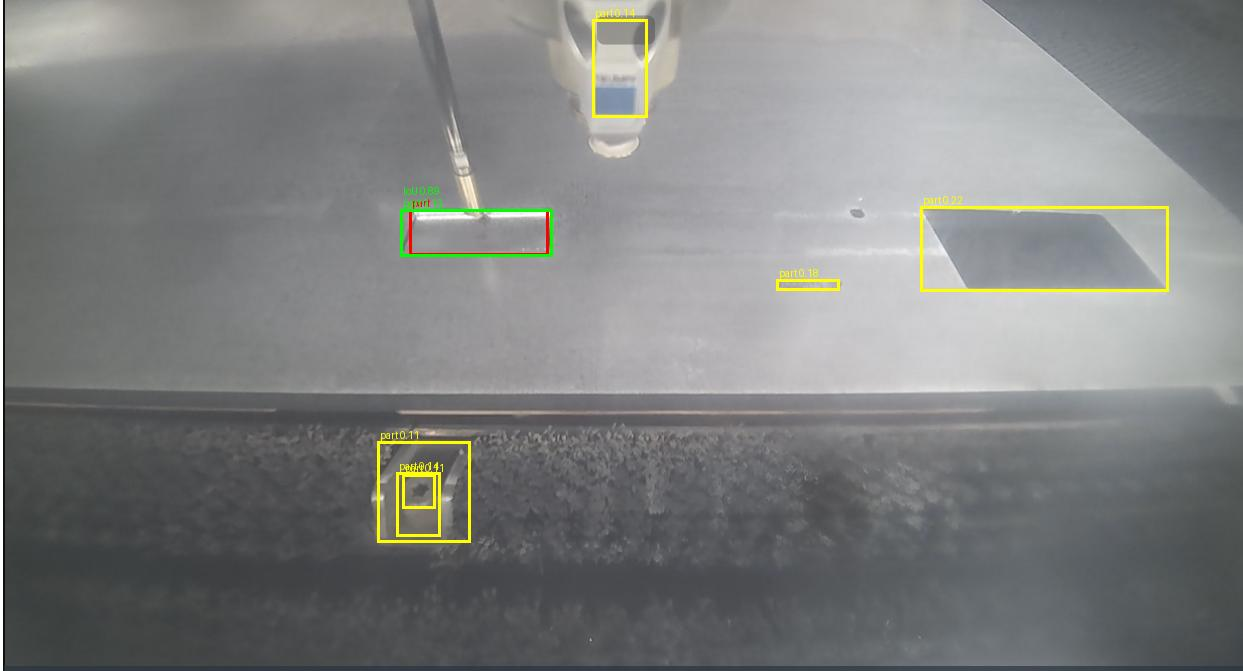
\includegraphics[width=0.9\linewidth]{graphics/example_synthetic_images/Beispiel_Detektion_rtdetr.jpg}
      \caption{Visualisierung einer Vorhersage des \ac{RT-DETR}-Modells mit Datenaugmentierung auf einem realen Bild (\textit{Confidence Threshold 0.1})}
      \label{fig:beispiel_vorhersage_rtdetr}
\end{figure}

\subsection{Zusammenfassung der Evaluationsergebnisse}
Es lässt sich zusammenfassen, dass die \ac{YOLO}-Modelle auf dem synthetischen Datensatz eine gute Leistung erbringen konnten, wobei alle drei Modelle in ihrer Leistung keine signifikanten Unterschiede aufwiesen. Das transformerbasierte Modell hingegen zeigte sowohl auf dem synthetischen als auch auf dem realen Datensatz eine deutlich schlechtere Leistung, trotz dass beide Varianten während des Trainings überraschend schnell konvergierten. Alle traininierten \ac{KI}-Modelle zeigten Schwierigkeiten bei der Übertragung ihrer Leistung auf realen Anwendungsfälle, was den Einfluss des \textit{Domain Gaps} verdeutlicht. Das \ac{YOLO}-Medium-Modell konnte dabei noch die beste Leistung auf dem realen Datensatz erzielen, erbrachte jedoch dennoch keine zufriedenstellende Leistung.
